\documentclass[12pt]{scrartcl}

\setlength{\parindent}{0pt}
\setlength{\parskip}{.25cm}

\usepackage{graphicx}

\usepackage{xcolor}

\definecolor{darkred}{rgb}{0.5,0,0}
\definecolor{darkgreen}{rgb}{0,0.5,0}
\usepackage{hyperref}
\hypersetup{
  letterpaper,
  colorlinks,
  linkcolor=red,
  citecolor=darkgreen,
  menucolor=darkred,
  urlcolor=blue,
  pdfpagemode=none,
  pdftitle={Lab 5.0 - Functions},
  pdfauthor={Christopher M. Bourke}
}

\definecolor{MyDarkBlue}{rgb}{0,0.08,0.45}
\definecolor{MyDarkRed}{rgb}{0.45,0.08,0}
\definecolor{MyDarkGreen}{rgb}{0.08,0.45,0.08}

\definecolor{mintedBackground}{rgb}{0.95,0.95,0.95}
\definecolor{mintedInlineBackground}{rgb}{.90,.90,1}

%\usepackage{newfloat}
\usepackage[newfloat=true]{minted}
\setminted{mathescape,
               linenos,
               autogobble,
               frame=none,
               framesep=2mm,
               framerule=0.4pt,
               %label=foo,
               xleftmargin=2em,
               xrightmargin=0em,
               startinline=true,  %PHP only, allow it to omit the PHP Tags *** with this option, variables using dollar sign in comments are treated as latex math
               numbersep=10pt, %gap between line numbers and start of line
               style=default, %syntax highlighting style, default is "default"
               			    %gallery: http://help.farbox.com/pygments.html
			    	    %list available: pygmentize -L styles
               bgcolor=mintedBackground} %prevents breaking across pages
               
\setmintedinline{bgcolor={mintedBackground}}
\setminted[text]{bgcolor={mintedBackground},linenos=false,autogobble,xleftmargin=1em}
%\setminted[php]{bgcolor=mintedBackgroundPHP} %startinline=True}
\SetupFloatingEnvironment{listing}{name=Code Sample}
\SetupFloatingEnvironment{listing}{listname=List of Code Samples}

\title{CSCE 155 - C}
\subtitle{Lab 5.0 - Functions}
\author{~}
\date{~}

\begin{document}

\maketitle

\section*{Prior to Lab}

Before attending this lab:
\begin{enumerate}
  \item Read and familiarize yourself with this handout.
  \item Read Chapters 5 and 18 of the \href{http://cse.unl.edu/~cbourke/ComputerScienceOne.pdf}{Computer Science I} textbook
  \item Watch Videos 5.1 thru 5.6 of the \href{https://www.youtube.com/playlist?list=PL4IH6CVPpTZVkiEnCEOdGbYsFEdtKc5Bx}{Computer Science I} video series
\end{enumerate}

\section*{Peer Programming Pair-Up}

\textbf{For students in the online section:} you may complete
the lab on your own if you wish or you may team up with a partner
of your choosing, or, you may consult with a lab instructor to get
teamed up online (via Zoom).

\textbf{For students in the face-to-face section:} your
lab instructor will team you up with a partner.  

To encourage collaboration and a team environment, labs are be
structured in a \emph{peer programming} setup.  At the start of
each lab, you will be randomly paired up with another student 
(conflicts such as absences will be dealt with by the lab instructor).
One of you will be designated the \emph{driver} and the other
the \emph{navigator}.  

The navigator will be responsible for reading the instructions and
telling the driver what to do next.  The driver will be in charge of the
keyboard and workstation.  Both driver and navigator are responsible
for suggesting fixes and solutions together.  Neither the navigator
nor the driver is ``in charge.''  Beyond your immediate pairing, you
are encouraged to help and interact and with other pairs in the lab.

Each week you should alternate: if you were a driver last week, 
be a navigator next, etc.  Resolve any issues (you were both drivers
last week) within your pair.  Ask the lab instructor to resolve issues
only when you cannot come to a consensus.  

Because of the peer programming setup of labs, it is absolutely 
essential that you complete any pre-lab activities and familiarize
yourself with the handouts prior to coming to lab.  Failure to do
so will negatively impact your ability to collaborate and work with 
others which may mean that you will not be able to complete the
lab.  

\section{Lab Objectives \& Topics}
At the end of this lab you should be familiar with the following:
\begin{itemize}
  \item Understand how to design, write, and use functions
  \item Know the difference between a function prototype and function definition
  \item Modularity and using separate header and source files
  \item Design test cases and write informal unit tests
\end{itemize}

\section{Background}

Most programming languages allow you to define and use functions 
(or methods).  Functions \emph{encapsulate} functionality into a 
unit of code that can be reused.  A function can be specified to 
take any number of inputs (called parameters or arguments) and 
return an output.  Defining and using functions has several advantages.  
First, it facilitates code reuse.  Rather than 
cutting and pasting a block of code, it can be encapsulated 
into a function and reused by calling the function anytime it needs 
to be executed.

Second, functions facilitate \emph{procedural abstraction}.  Often, 
we don't care or need to worry about the implementation 
details of a certain algorithm or procedure.  By encapsulating the 
details in a function, we only need to know how to use it (what 
inputs to provide it and what output we can expect from it).  We
don't need to worry about \emph{how} it computes its result.  For example,
up to now you've been using the standard math library's function
to compute the square root of a number $x$, but you haven't
had to worry about the details of how this computation actually
takes place.

Finally, functions naturally define a \emph{unit} of code that can
be easily tested.  Typically, unit tests are designed with 
\emph{test cases} which are input/output combinations that are
known to be correct.  Unit testing involves feeding the input to
a function and comparing the output to the \emph{expected} output.
If they match, we say the test case \emph{passes}, if not, we say
it \emph{fails}.  Unit testing gives a higher level of confidence
that our function's implementation is correct.

When defining a function, it is necessary to declare its \emph{signature}.  
The signature of a function includes:
\begin{itemize}
  \item The function's identifier -- its name 
  \item The return type -- the type of variable the function returns
  \item The parameter list -- the number of parameters the function takes 
	(also called its \emph{arity}) along with their types 
\end{itemize}

\subsection{Functions in C}

In C, functions must be declared before they can be defined or used.  
Functions are declared by defining \emph{prototypes}: a 
declaration of the function's signature followed by a semicolon.  
Prototypes are usually placed into separate header files (with file
names ending in \mintinline{text}{.h}) and their definitions are
placed into source files with the same base name (but ending in 
\mintinline{text}{.c}).  Function definitions repeat the signature 
but are followed by a block of code that specifies the 
instructions that will be executed when the function is called or
\emph{invoked}.

\section{Activities}

We have provided partially completed programs for each of the 
following activities.  Clone the lab's code from GitHub using the 
following URL: \url{https://github.com/cbourke/CSCE155-C-Lab05}.

\subsection{Using Functions}

The file \mintinline{text}{orderStatistic.c} contains code necessary
to find the $i$-th order statistic of a collection of numbers.   
The $i$-th order statistic corresponds to the $i$-th element in a 
sorted list.  For example, the 4th order statistic of the list 
[5, 99, 23, 14, 6] is 23; the sorted list is [5, 6, 14, 23, 99], 
and 23 is the 4th element.  Some special cases:
\begin{itemize}
  \item The 1-th order statistic is the \emph{minimum} element
  \item The $n$-th order statistic is the \emph{maximum} element
  \item The $\frac{n}{2}$-th order statistic is the \emph{median} element
\end{itemize}
The program converts command line arguments into $i$ and an
array of integers.  It then sorts the array and outputs the $i$-th 
element.  It does so by calling a series of functions.

\subsubsection*{Instructions}

\begin{enumerate}
  \item Manually compile the order statistics program:
  \begin{enumerate}
    \item Compile the order statistics ``library'' using the following: \\
    \mintinline{text}{gcc -c -std=gnu99 orderStatistics.c} 
    
    The \mintinline{text}{-c} flag tells gcc to compile (without linking)
    which produces an \emph{object} file \mintinline{text}{orderStatistics.o}.
    This is not an executable program, but contains compiled code of
    the functions in \mintinline{text}{orderStatistics.c}
    \item Compile your executable and \emph{link} it to this ``library''
    using the following: \\
    \mintinline{text}{gcc orderStatistics.o orderStatisticsDemo.c}
  \end{enumerate}
  \item Run the program with the following input values and verify
  that it is correct: \\
	\mintinline{text}{./a.out 4 99 23 76 100 8 3 0 1 72 104 1000 12 18 14}
  \item Complete questions 1 and 2 on your worksheet.
\end{enumerate}

\subsection{Writing Functions}

Images are made up of individual \emph{pixels}.  Each pixel can be 
represented using an RGB (red-blue-green) color scheme.  RGB is 
generally used in displays and models a color with three integer 
values in the range $[0, 255]$ corresponding to the red, green and 
blue ``contribution'' to the color.  For example, the triple 
$(255, 255, 0)$ corresponds to a full red and green (additive) value
which results in yellow.  

Two common image filters are a black-and-white filter which transforms
an image into an equivalent gray-scale image, and a sepia filter which
transforms a photo to a reddish-brown monochrome to give it an old-timey
look.

We have already written a substantial program that processes an image
file and applies one of these filters.  However, you will need to write
the functions responsible for transforming an RGB value into a gray-scale
or sepia RGB value.  

To convert an RGB value to gray-scale you can use one of several
different techniques.  Each technique ``removes'' the color value by
setting all three RGB values to the same value but each technique 
does so in a slightly different way.

The first technique is to simply take the average of all three values:
  $$\frac{r + g + b}{3}$$

The second technique, known as the ``lightness'' technique averages 
the most prominent and least prominent colors:
  $$\frac{\max\{r, g, b\} + \min\{r, g, b\}}{2}$$

The luminosity technique uses a weighted average to account for a human 
perceptual preference toward green, setting all three values to:
  $$0.21 r + 0.72 g + 0.07 b$$

\textbf{Note}: in all three cases, the final value should be
\emph{rounded} before being returned (\emph{not} truncated).

A sepia filter sets different values to each of the three RGB components 
using the following formulas.  Given a current $(r,g,b)$ value, the sepia
tone RGB value, $(r',g',b')$ would be:
$$\begin{array}{ll}
  r' &= 0.393r + 0.769g + 0.189b \\
  g' &= 0.349r + 0.686g + 0.168b \\
  b' &= 0.272r + 0.534g + 0.131b
\end{array}$$
As with the gray-scale techniques, the final values should be rounded.  
Moreover, if any of the values exceeds 255, they should be reset to 255 to stay within
the valid RGB color range.

\subsubsection*{Instructions}

Design and write a ``color utilities'' library by implementing the 
functions described below.  In particular:
\begin{itemize}
  \item Place your prototypes and documentation in the file
  \mintinline{text}{colorUtils.h}
  \item Place your function definitions in the file 
  \mintinline{text}{colorUtils.c}.  
  \item Your color library functions are used in an image manipulation
  program (already written for you) that converts images to 
  gray scale/sepia.  
  
  As software projects become more complex, the commands, rules, 
  and order that you compile
  files becomes complex.  A makefile codifies these rules and 
  automatically builds your entire project with a single command.
  
  We've provided a \mintinline{text}{makefile} which defines the rules
  and dependencies required to build the image manipulation 
  program. From the command line, simply type 
  
  \mintinline{text}{make} 
  
  and it will produce an
  executable called \mintinline{text}{imageDriver}.  
  
  \item Run the \mintinline{text}{imageDriver} program on the images
  we've provided as part of the project, or you can upload your own
  images and play around with this program.  If your functions
  are correctly, the image conversion should look something like 
  Figure \ref{fig:imageComparisons}.
\end{itemize}

\begin{figure}[h]
\centering
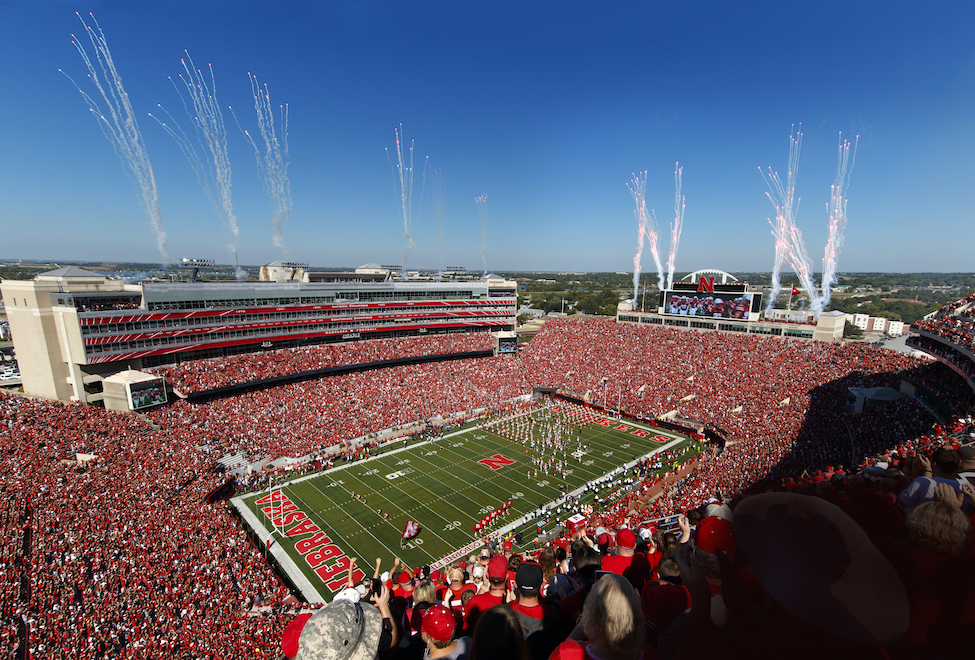
\includegraphics[scale=0.20]{../memorialStadium}
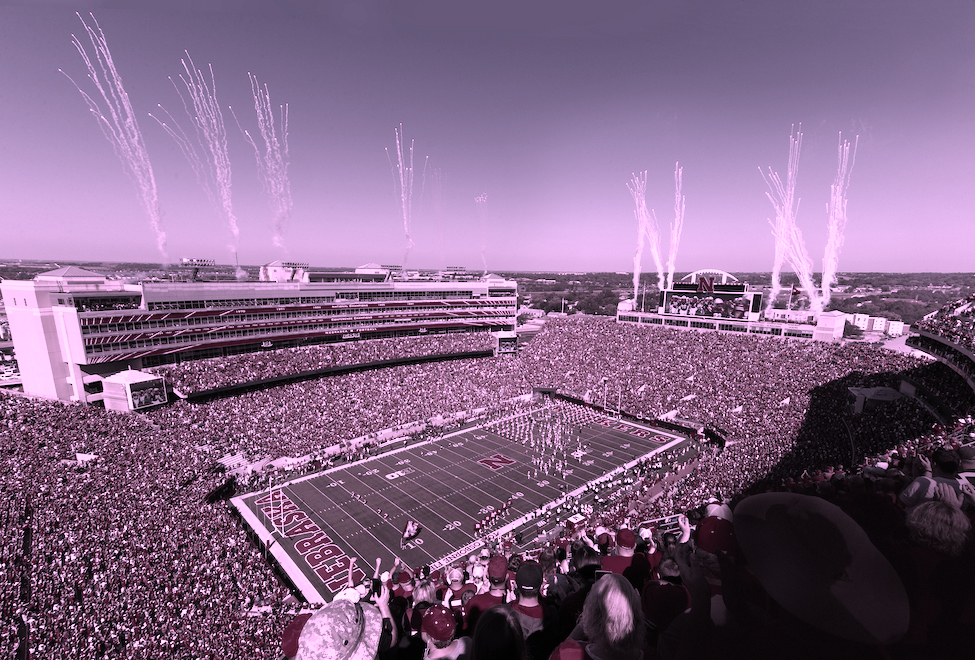
\includegraphics[scale=0.20]{../memorialStadiumSepia}
\caption{Memorial Stadium.  Original image (left) and Sepia-toned image (right).}
\label{fig:imageComparisons}
\end{figure}

We've provided starter code with two functions already completed for
you.  Implement the following functions:

\begin{itemize}
  \item Write a helper function that returns the \emph{minimum}
  of 3 integers.  Name your function \mintinline{c}{min}.
  
  \item Write a function that takes three integer values (RGB values) and
  uses the lightness technique to return the gray-scale value.  
  Name your function \mintinline{c}{toGrayScaleLightness}

  \item Write a function that takes three integer values (RGB values) and
  uses the luminosity technique to return the gray-scale value.  
  Name your function \mintinline{c}{toGrayScaleLuminosity}

  \item Write three functions to compute the three sepia-tone RGB values.
  You'll need three functions because a function can only return one value.
  Name your functions \mintinline{c}{toSepiaRed}, \mintinline{c}{toSepiaGreen} and
  \mintinline{c}{toSepiaBlue} respectively.
\end{itemize}


\subsection{Writing Tests}

Testing is a fundamental step in software development.  The most common types
of tests are \emph{unit tests} and the most common ``unit'' is a function.
You may have already ``tested'' your functions by running the project and 
viewing the resulting images.  However, for your final activity, you will
write more automatable unit tests to test your functions more rigorously.  

Some starter unit testing code has already been provided in 
\mintinline{text}{colorUtilsTester.c}.  Each block of code calls a function
with some inputs and compares the return value to the \emph{expected}
output.  If they match, the test passes, if not it fails.  A message is
printed to the user and the total number of passed/failed test cases is
reported.  

Using this starter code as an example, add more test cases for the 
other functions.  You should write at least 1 test case for 
\emph{each} function you wrote.  

To compile this tester you can use the same make file and the
following:

\mintinline{text}{make colorUtilsTester}

which produces an executable program called \mintinline{text}{colorUtilsTester}

\section{Handin/Grader Instructions}

\begin{enumerate}
  \item Hand in your completed files:
  \begin{itemize}
    \item \mintinline{text}{colorUtils.c}
    \item \mintinline{text}{colorUtils.h}
    \item \mintinline{text}{colorUtilsTester.c}
    \item \mintinline{text}{worksheet.md}
  \end{itemize}
  through the webhandin (\url{https://cse-apps.unl.edu/handin}) 
  using your cse login and password.  
  \item Even if you worked with a partner, you \emph{both} should
  turn in all files.
  \item Verify your program by grading yourself through the
  webgrader (\url{https://cse.unl.edu/~cse155e/grade/}) using the
  same credentials.
  \item Recall that both expected output and your program's output
  will be displayed.  The formatting may differ slightly which is fine.
  As long as your program successfully compiles, runs and outputs 
  the \emph{same values}, it is considered correct.
\end{enumerate}

\section{Advanced Activity (Optional)}

Large projects require even more abstraction and tools to manage 
source code and specify how it gets built.  One tool to facilitate this 
is a program called Make which uses makefiles--specifications for 
which pieces of code depend on other pieces and how all pieces 
get built and combined to build an executable program (or collection 
of executables).  The use of modern IDEs has made the build process 
much more manageable, but make is still widely used.  Several 
useful tutorials exist describing how makefiles can be defined and 
used.
\begin{itemize}
  \item \url{http://www.opussoftware.com/tutorial/TutMakefile.htm}
  \item \url{http://mrbook.org/tutorials/make/}
\end{itemize}
We have provided a makefile for this lab.  Read through the tutorials
above and then read through the makefile and understand how it works.
Write your own makefile for your next assignment to simplify the
compilation process.


\end{document}
